
Note that the many of the formulas and algorithms referenced in the 
report are from the course notes.

\section*{Q1: Dynamic programming}
\subsection*{1}
Policy Iteration was used here - policy iteration was chosen as 
it is in general faster.
A small tolerance ($tolerance = 0.00001$) was set for the 
stopping condition of the policy evaluation step. This 
tolerance was chosen to be small enough as to confirm convergence 
of the policy evaluation. Especially as the rewards are to the 
nearest integer the tolerance is sufficiently small.

The Policy Iteration implementation is split into two
stages: the policy evaluation and the policy improvement stages.
Both of these are wrapped in a while loop that only terminates 
when the policy improvement stage does not update the policy 
(the flag $policy_stable$ is set to false if the policy is updated
in policy improvement; otherwise is true and will terminate).

For the policy evaluation, $\Delta$ is initialised to $10 * \theta$ 
where $\theta = tolerance$. This ensures that the policy evaluation
loop will be entered. 
There is a nested loop in Policy Evaluation, the outer one for looping 
through all available states and the inner for updating the value 
for the selected state, ie $V(s)$.
The optimal policy given a state for the current iteration $\pi(s)$,
is computed simply by finding the index with the largest value
in the policy matrix corresponding to state.
The current $V$ is cached as each state requires the original
$V(s')$ to be able update the current $V(s)$.
$P^{\pi(s)}_{s s'}$ is the value from the transition matrix. 
The reward $R^{\pi(s)}_{s s'}$ is also computed given $\pi(s)$.
% This ensures that only the chosen action has a non zero probility
% (note that the policy is greedy, so only one value in the policy should 
% be $1$). Note that the policy is initialised to such that each state
% starts with bias towards the value

The optimal policy (action) is determined for each state using a greedy
approach - the best policy after the update is the policy the action
that maximises the value of 
$\sum_{s'} P^a_{ss'}[R^a_{ss'} + \gamma V(s')]$ as defined in the lectures.
Here the policy is represented as a 2D matrix of shape 
$(number of states, number of actions)$. Each row of the matrix 
defines the policy of that given state by using a bit set where there 
is exactly one index with the value $1$ (and the rest is $0$) 
and a value of $1$ at an index means that given index is the optimal
policy for that state. 

Note that the initialisation of $\pi(s)$ is set to $[0,1,0,0]$ which 
represents the starting policy for each state pointing east.
This is arbitary and mainly set to satisfy the above design of the 
policy - each row much have exactly a single $1$. 

% TODO: finish this section

\subsection*{2}
\begin{figure}[H]
    \centering
    \begin{subfigure}[b]{0.49\textwidth}
        \centering
        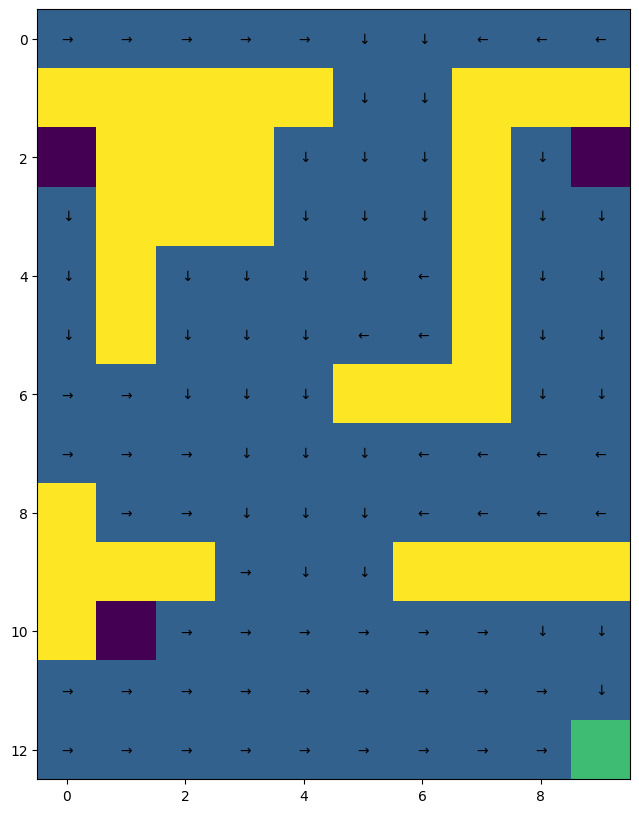
\includegraphics[width=\textwidth]{assets/dp/dp_optimal_policy.png}        
        \caption{Dynamic Programming Policy}
    \end{subfigure}
    \hfill 
    \begin{subfigure}[b]{0.49\textwidth}
        \centering
        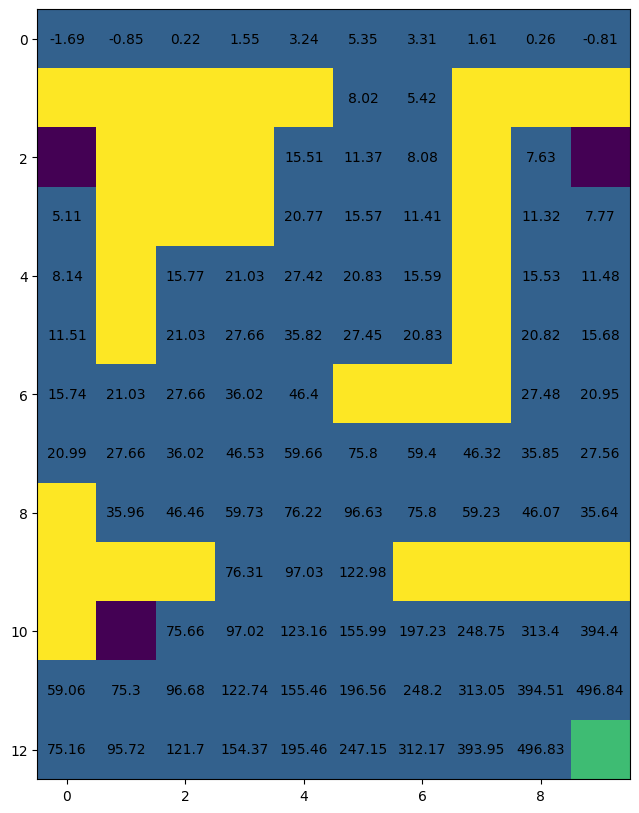
\includegraphics[width=\textwidth]{assets/dp/dp_value_function.png}        
        \caption{Dynamic Programming Value FUnction}
    \end{subfigure}
    \caption*{Graphical Representations of Dynamic Programming Results}
\end{figure} 

% \break
\subsection*{3}

\begin{landscape}
\begin{center}
    \begin{tabular}{c || c  c  c}
        & & $\gamma$ & \\
        & 0.1 & 0.25 & 0.5 \\
        \hline \hline \\
        0.2 & 
            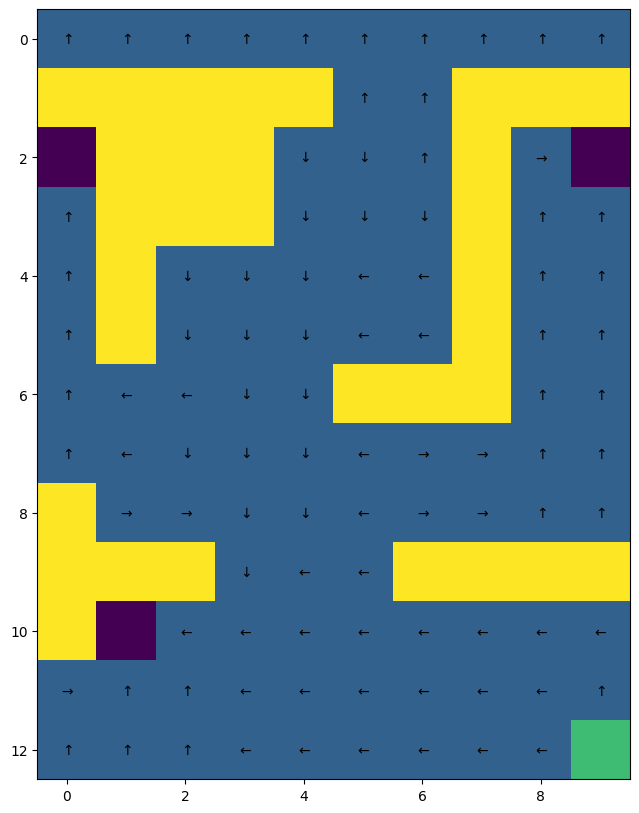
\includegraphics[width=0.35\textheight]{assets/dp/analysis/prob_0.1_gamma_0.2_policy.png}
        & 
            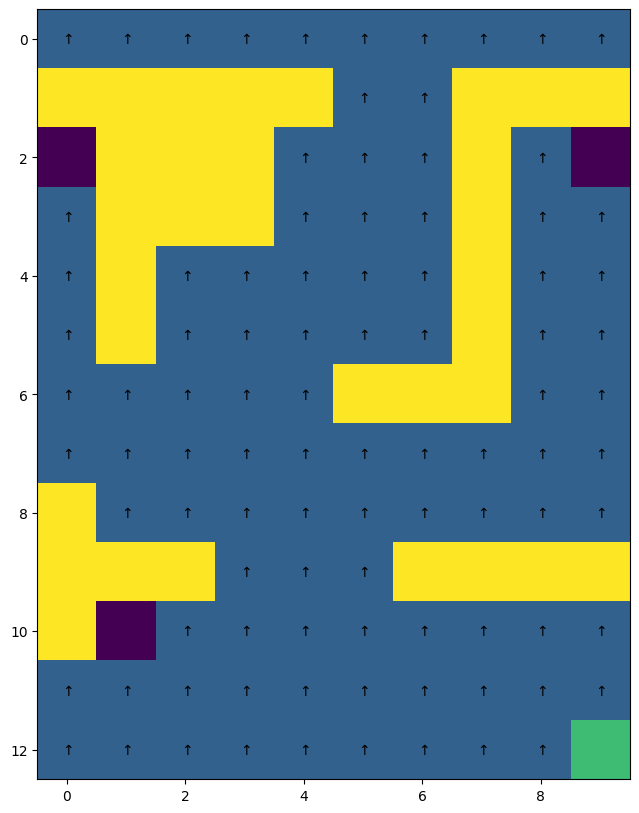
\includegraphics[width=0.35\textheight]{assets/dp/analysis/prob_0.25_gamma_0.2_policy.png}
        & 
            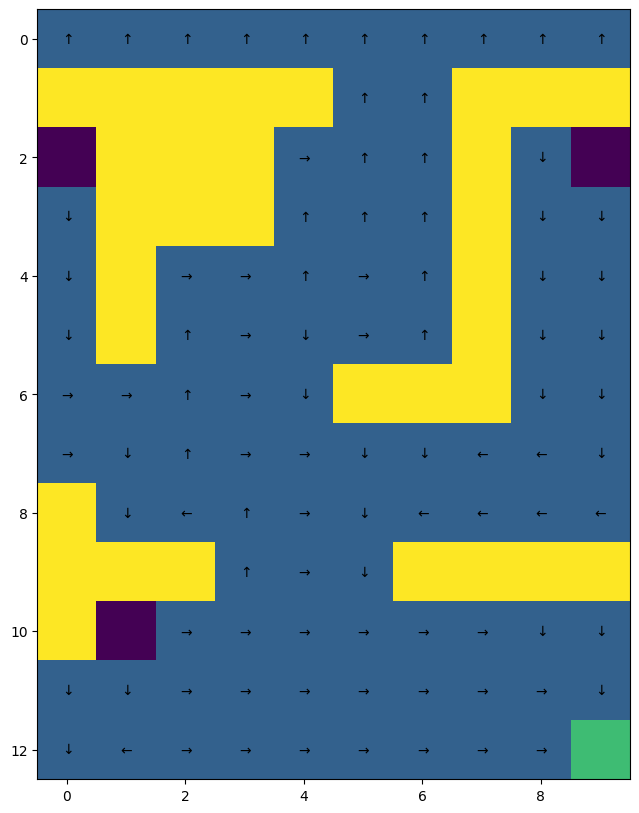
\includegraphics[width=0.35\textheight]{assets/dp/analysis/prob_0.5_gamma_0.2_policy.png}
        \\
        0.8 &
            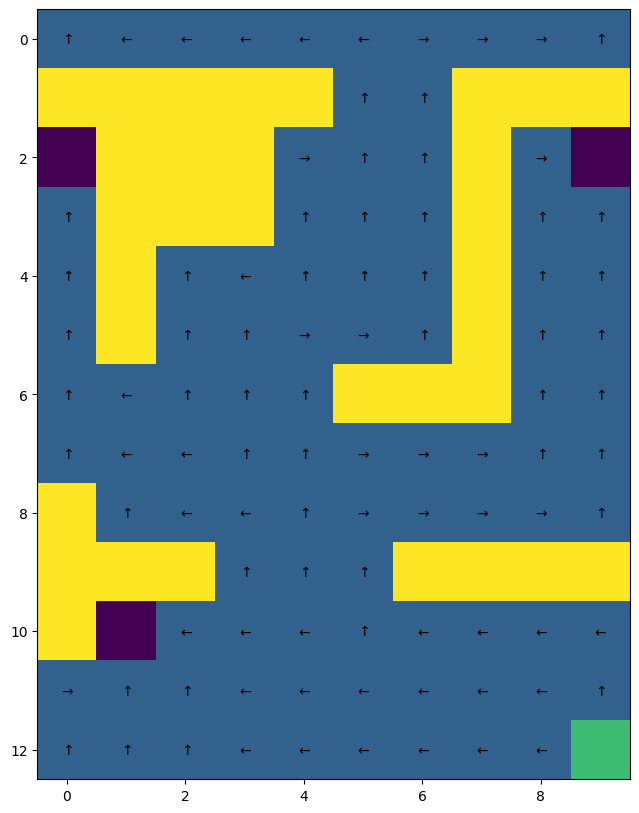
\includegraphics[width=0.35\textheight]{assets/dp/analysis/prob_0.1_gamma_0.8_policy.png}
        & 
            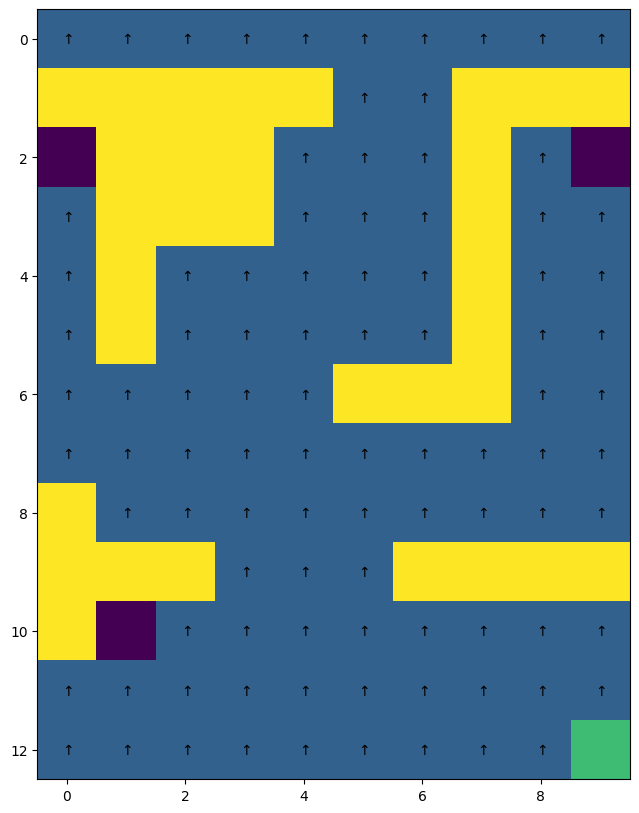
\includegraphics[width=0.35\textheight]{assets/dp/analysis/prob_0.25_gamma_0.8_policy.png}
        &
            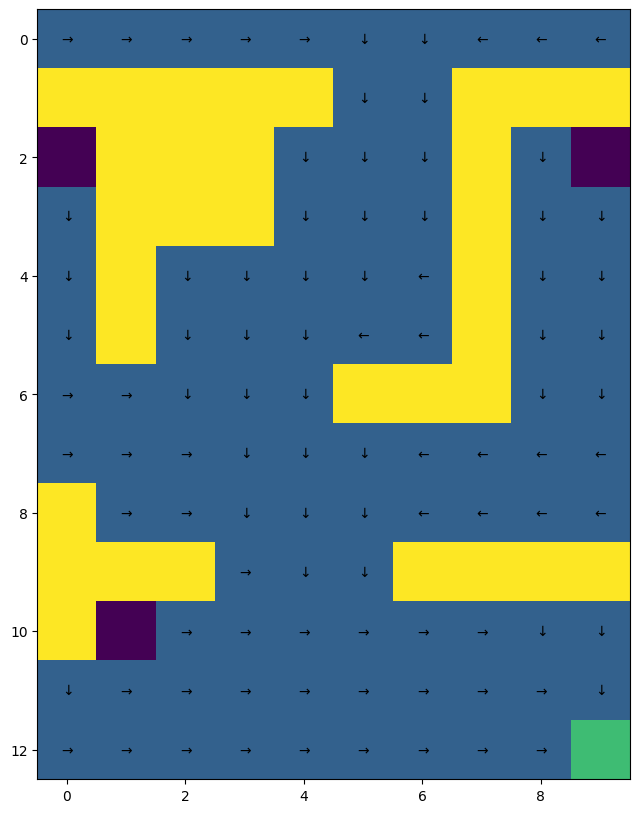
\includegraphics[width=0.35\textheight]{assets/dp/analysis/prob_0.5_gamma_0.8_policy.png}
    \end{tabular}        
\end{center}

\begin{center}
    \begin{tabular}{c || c  c  c}
        & & $\gamma$ & \\
        & 0.1 & 0.25 & 0.5 \\
        \hline \hline \\
        0.2 & 
            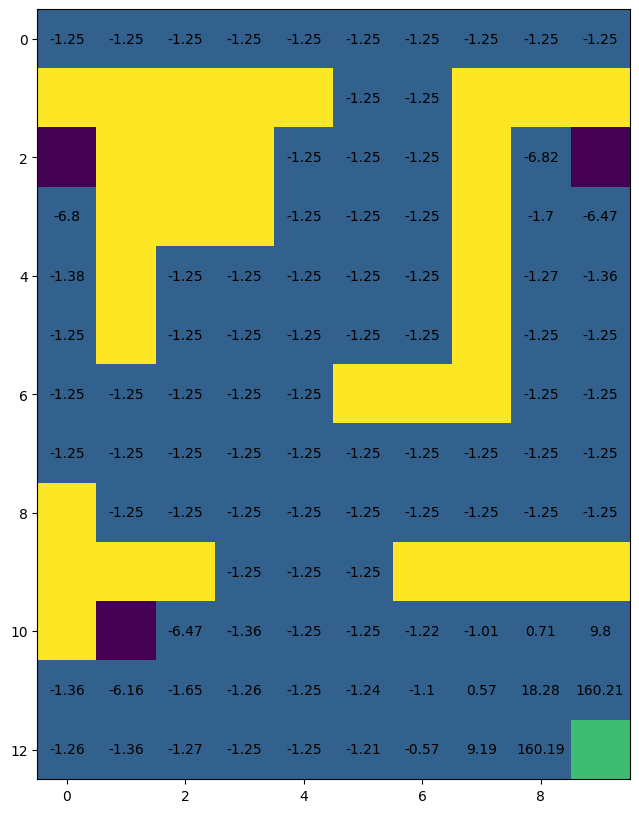
\includegraphics[width=0.35\textheight]{assets/dp/analysis/prob_0.1_gamma_0.2_value.png}
        & 
            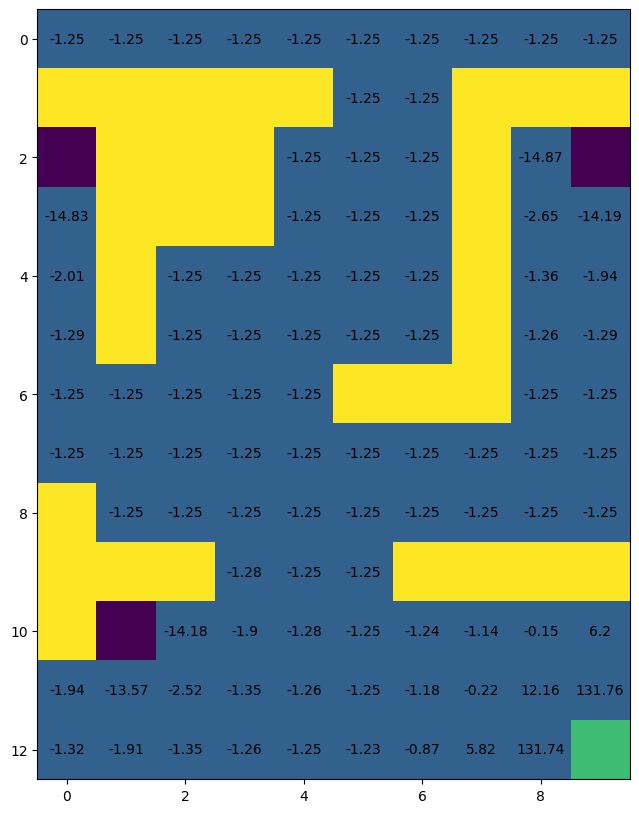
\includegraphics[width=0.35\textheight]{assets/dp/analysis/prob_0.25_gamma_0.2_value.png}
        & 
            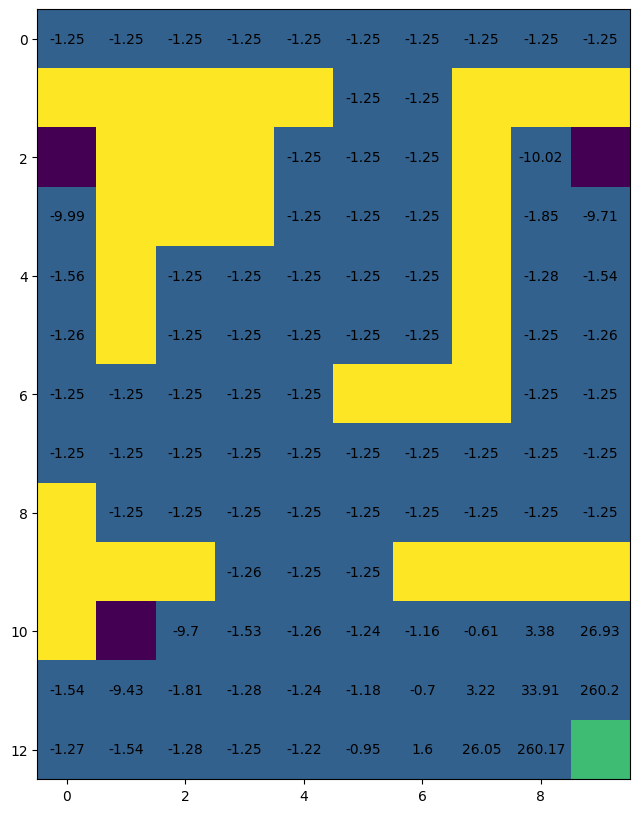
\includegraphics[width=0.35\textheight]{assets/dp/analysis/prob_0.5_gamma_0.2_value.png}
        \\
        \centering 0.8 &
            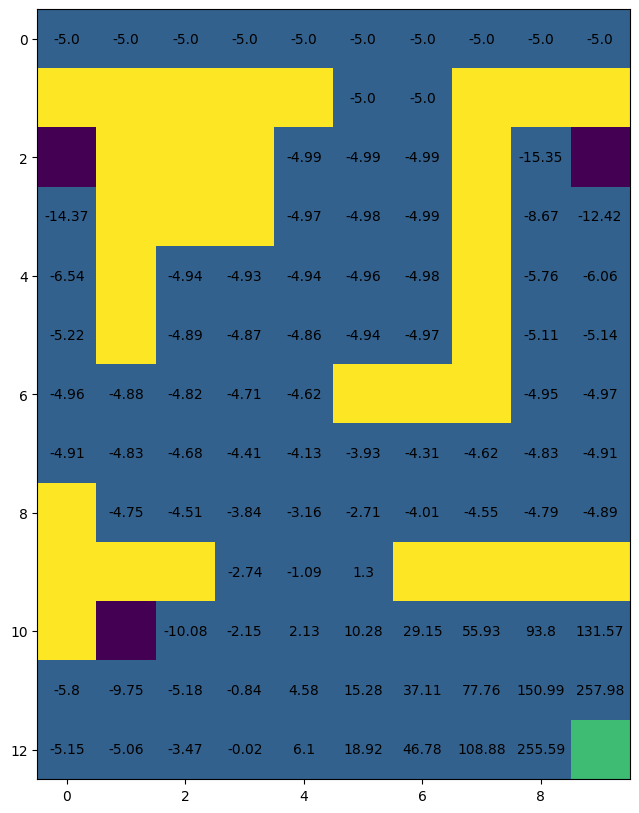
\includegraphics[width=0.35\textheight]{assets/dp/analysis/prob_0.1_gamma_0.8_value.png}
        & 
            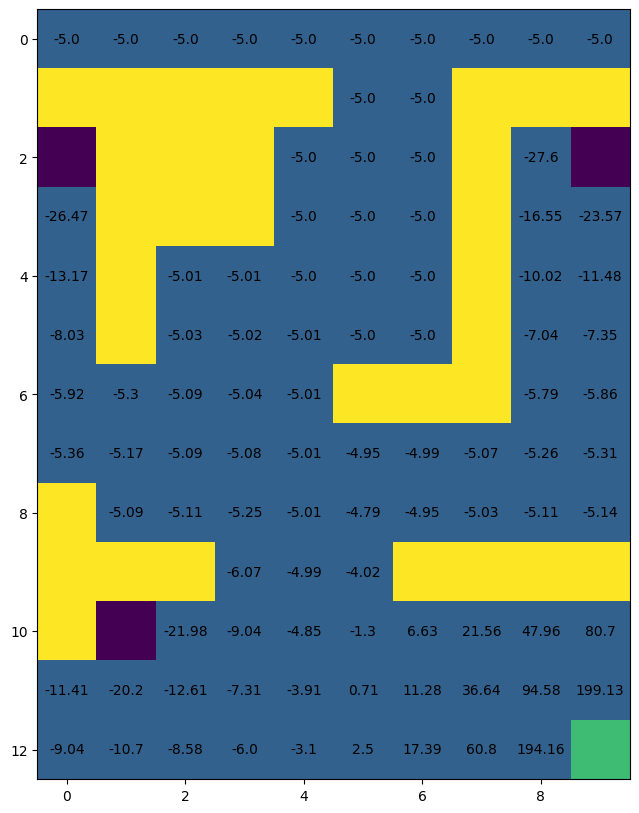
\includegraphics[width=0.35\textheight]{assets/dp/analysis/prob_0.25_gamma_0.8_value.png}
        &
            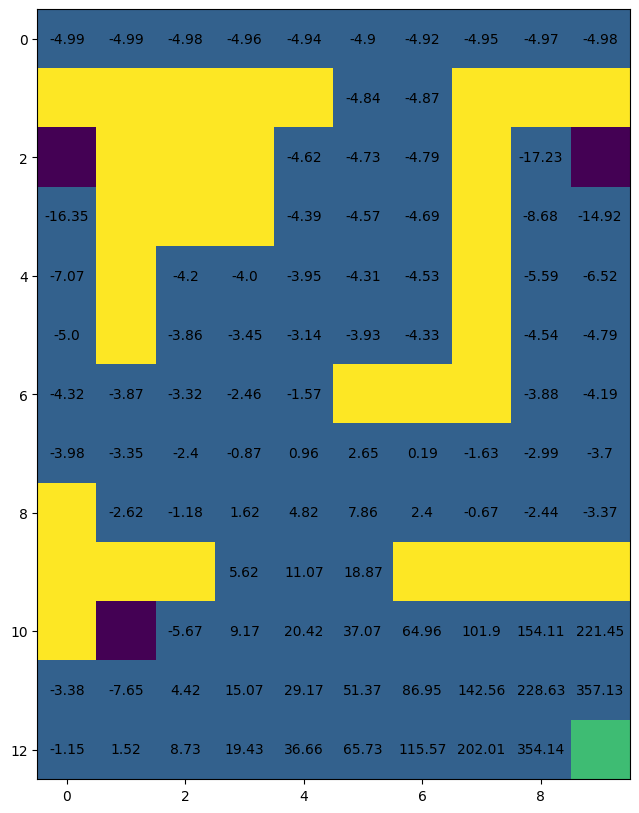
\includegraphics[width=0.35\textheight]{assets/dp/analysis/prob_0.5_gamma_0.8_value.png}
    \end{tabular}        
\end{center}
\end{landscape}
\break

When the probability $p = 0.25$, the transition matrix probability
of success is $0.25$ and the probability of going in another direction
is also $0.25$.
Both diagrams at $p = 0.25$ show that the policy $\pi(s) = North \forall s \in S$.
This is to be expected as
$ \forall s, s' \in \mathcal{S}, \forall a \in \mathcal{A}, P^a_{ss'} = 0.25$ given 
the previous conditions. 

Consider the value evaluation 
$V(s) \leftarrow \max_a \sum_{s'} P^a_{ss'}[R^a_{ss'} + \gamma V(s')]$
the policy update $\pi(s) \leftarrow argmax_a \sum_{s'} P^a_{ss'}[R^a_{ss'} + \gamma V(s')]$.
Both become $V(s) \leftarrow \frac{1}{4}\max_a \sum_{s'} [R^a_{ss'} + \gamma V(s')]$
and $\pi(s) \leftarrow argmax_a \sum_{s'} [R^a_{ss'} + \gamma V(s')]$
respectively.
In this problem, $R^a_{ss'} = R^b_{ss'}, \forall a, b \in \mathcal{A}$. 
As such, it can be seen that the policy update of $\pi(s)$ is 
not effected by the value of the action chosen. Since numpy's
$argmax$ function is chosen to be used to update the function, 
it chooses the lowest index which in this case is $0$ and corresponds
to the action $North$. 

Now consider when $p < 0.25$.
In this scenario, the probability of successfully traversing the the
optimal direction is the least out of all the possible actions.
As such, instead of the policy determining the optimal path from the
start to the end point, the policy can be interpreted as the worst
or least optimal action. This can clearly be seen from the flow 
of the arrows, point away from the goal state and pointing to either
the start states or other absorbing states. 

When $p > 0.25$, the behaviour is as expected: the policy derived
is the expected optimal path to the end point.
% This results in moving in another direction the same probability 
% as the current optimal policy. Consider the policy update $\pi(s) \leftarrow
% argmax_a \sum_{s'} P^a_{ss'}[R^a_{ss'} + \gamma V(s')]$: the value $P^a_{ss'}$ 
% will be biggest when the 
% % TODO
% (When $p < 0.25$ this effect is exaggerated and the expected policy 
% is not achieved.)

The value of $\gamma$ does not significantly affect the 
result of the policy.
However it does effect the resultant value function:
lower gamma, results in lower the value function having a smaller 
range. This is to be expected given the value update is given by 
$V(s) \leftarrow \max_a \sum_{s'} P^a_{ss'}[R^a_{ss'} + \gamma V(s')]$.
Small $\gamma$ means the impact of $V(s')$ is smaller resulting the 
the behaviour seen.